\documentclass[11pt,class=report,crop=false]{standalone}
\usepackage[screen]{../python}

\begin{document}

%====================================================================
\chapitre{Python : numpy et matplotlib avec une variable}
%====================================================================

\insertvideo{2sO3d1s2wPk}{partie 2.1. Numpy}

\insertvideo{IuEY3K_RroI}{partie 2.2. Matplotlib}


\objectifs{Le but de ce court chapitre est d'avoir un aperçu de deux modules \Python{} :
\numpy{} et \matplotlib{}. Le module \numpy{} aide à effectuer des calculs numériques efficacement.
Le module \matplotlib{} permet de tracer des graphiques.}

\bigskip

Ce chapitre est un chapitre plutôt technique, il suppose une connaissance de base de \Python.
Dans un premier temps, nous allons uniquement nous intéresser aux fonctions d'une variable.
Il faut prendre garde à ne pas trop s'attarder sur les détails et les multiples fonctionnalités de ces deux modules. Vous pourrez revenir vers ce chapitre en fonction de vos besoins futurs.

Voici un aperçu du code le plus simple que l'on puisse écrire pour tracer une fonction.
Il s'agit de tracer le graphe de la fonction $x \mapsto \cos(x)$ sur $[0,10]$.

\begin{minipage}{0.45\textwidth}
\begin{lstlisting}
import numpy as np
import matplotlib.pyplot as plt

X = np.linspace(0,10,num=100)
Y = np.cos(X)

plt.plot(X,Y)
plt.show()
\end{lstlisting}
\end{minipage}
\begin{minipage}{0.49\textwidth}
\begin{center}
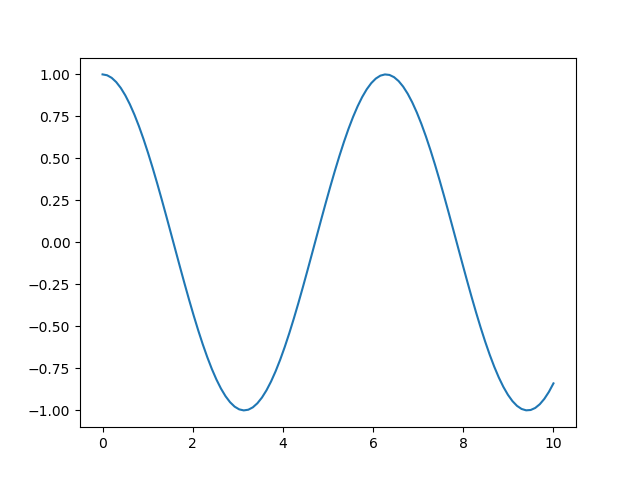
\includegraphics[scale=\myscale,scale=0.55]{figures/pythonx-intro}
\end{center}
\end{minipage}

Attention ! \numpy{} et \matplotlib{} ne sont pas toujours installés avec votre distribution \Python. Vous devrez peut-être les installer vous-même.


%%%%%%%%%%%%%%%%%%%%%%%%%%%%%%%%%%%%%%%%%%%%%%%%%%%%%%%%%%%%%%%%%%%%%
\section{Numpy (une variable)}

On appelle le module \numpy{} et on le renomme de façon raccourcie \og{}\ci{np}\fg{} :
\mycenterline{\ci{import numpy as np}}

%--------------------------------------------------------------------
\subsection{Définition d'un vecteur}

Les principaux objets de  \numpy{} sont des \og{}tableaux\fg{}. Dans ce chapitre nous étudierons seulement les tableaux à une dimension que l'on appelle des \defi{vecteurs}.

\begin{itemize}
  \item Définition à partir d'une liste : 
\mycenterline{\ci{X = np.array([1,2,3,4])}}
  \item Affichage par \ci{print(X)} :
\mycenterline{\ci{[1 2 3 4]}}
 
   Cela ressemble beaucoup à une liste, mais ce n'est pas une liste usuelle de \Python.
   Le type de \ci{X} est \ci{numpy.ndarray}.
   Notez qu'il n'y a pas de virgules dans l'affichage du vecteur.
   
 
  \item Définition d'une suite d'éléments avec \ci{arange()}\index{numpy@\numpy!arange@\ci{arange()}}. Cette fonction a le même comportement que la fonction classique \ci{range()} avec en plus la possibilité d'utiliser un pas non entier.
  Par exemple : 
  \mycenterline{\ci{np.arange(1,8,0.5)}}
  renvoie :
  \mycenterline{\ci{[1.  1.5  2.  2.5  3.  3.5  4.  4.5  5.  5.5  6.  6.5  7.  7.5]}}
  
  \item Définition d'une division d'intervalle avec \ci{linspace()}\index{numpy@\numpy!lonspace@\ci{linspace()}}. C'est l'une des méthodes les plus utilisées. Elle s'utilise avec la syntaxe \ci{linspace(a,b,num=n)} pour obtenir une subdivision régulière de $[a,b]$ de $n$ valeurs (donc en $n-1$ sous-intervalles). Exemple :
  \mycenterline{\ci{np.linspace(0,1,num=12)}}
  vaut :
  \begin{center}
  \begin{minipage}{0.9\textwidth}
\begin{lstlisting}
[0.         0.09090909 0.18181818 0.27272727 0.36363636 0.45454545
 0.54545455 0.63636364 0.72727273 0.81818182 0.90909091 1.        ]
\end{lstlisting}
  \end{minipage}
  \end{center}

\end{itemize}

%--------------------------------------------------------------------
\subsection{Opérations élémentaires}

Voici les opérations élémentaires utiles pour manipuler des vecteurs. Elles ont toutes la particularité d'agir sur les coordonnées.

Définissons un vecteur $X$ par :
\mycenterline{\ci{X = np.array([1,2,3,4])}}

\begin{itemize}
  \item Multiplication par un scalaire. Par exemple \ci{2*X} renvoie le vecteur \ci{[2 4 6 8]}.
  \item Addition d'une constante. Par exemple \ci{X+1} renvoie le vecteur \ci{[2 3 4 5]}.
  \item Carré. Par exemple \ci{X**2} renvoie le vecteur \ci{[1 4 9 16]}.
  \item Inverse. Par exemple \ci{1/X} renvoie le vecteur \ci{[1. 0.5 0.33333333 0.25]}.
  \item Somme. Par exemple \ci{np.sum(X)} renvoie le nombre $10$.
  \item Minimum, maximum. Par exemple \ci{np.min(X)} renvoie $1$ et \ci{np.max(X)} renvoie $4$.
\end{itemize}

\bigskip
 
Si $Y$ est un autre vecteur défini par \ci{Y = np.array([10,11,12,13])} alors :
\begin{itemize}
  \item Somme terme à terme. Par exemple \ci{X+Y} renvoie \ci{[11 13 15 17]}.
  \item Produit terme à terme. Par exemple \ci{X*Y} renvoie \ci{[10 22 36 52]}.
\end{itemize}


%--------------------------------------------------------------------
\subsection{Définition d'un vecteur (suite)}

Voici plusieurs façons d'initialiser un vecteur.
\begin{itemize}
  \item Avec des zéros. Exemple : \ci{np.zeros(5)} renvoie \ci{[0. 0. 0. 0. 0.]}\index{numpy@\numpy!zeros@\ci{zeros()}}.
  \item Avec des uns. Exemple : \ci{X = np.ones(5)}, alors \ci{X} vaut \ci{[1. 1. 1. 1. 1.]}.
  Ainsi \ci{7*X} renvoie \ci{[7. 7. 7. 7. 7.]}.\index{numpy@\numpy!ones@\ci{ones()}}
  \item Avec des nombres aléatoires entre $0$ et $1$. Exemple : \ci{np.random.random(5)} renvoie un vecteur dont les coordonnées sont tirées aléatoirement à chaque appel, on obtient par exemple :
  \mycenterline{\ci{[0.21132407 0.30685886 0.94111979 0.39597993 0.63275735]}}
  \index{numpy@\numpy!random@\ci{random()}}
\end{itemize}

%--------------------------------------------------------------------
\subsection{Utilisation comme une liste}

Prenons l'exemple du vecteur $X$ :
\mycenterline{\ci{[1.         1.11111111 1.22222222 1.33333333 1.44444444 1.55555556
 1.66666667 1.77777778 1.88888889 2.        ]}}
défini par la commande :
\mycenterline{\ci{X = np.linspace(1,2,num=10)}}

\begin{itemize}
  \item Récupérer une coordonnée. \ci{X[0]} renvoie le premier élément de \ci{X}, \ci{X[1]} renvoie le second élément, etc.
  
  \item Longueur d'un vecteur. \ci{len(X)} renvoie le nombre d'éléments. Une commande similaire est \ci{np.shape(X)}. 
  
  \item Parcourir tous les éléments. Deux méthodes :
  \begin{center}
\begin{minipage}{0.40\textwidth}
\begin{lstlisting}
for x in X:
  	print(x) 
\end{lstlisting}
\end{minipage}
  \begin{minipage}{0.40\textwidth}
\begin{lstlisting}
for i in range(len(X)):
	print(i,X[i])
\end{lstlisting}
  \end{minipage}
  \end{center}
\end{itemize}

%--------------------------------------------------------------------
\subsection{Application d'une fonction}

Avec \numpy{}, on peut appliquer une fonction directement sur chaque coordonnée d'un vecteur.

Prenons l'exemple de :
\mycenterline{\ci{X = np.array([0,1,2,3,4,5])}}

\begin{itemize}
  \item Racine carré. Par exemple \ci{np.sqrt(X)} renvoie le vecteur \ci{[0.         1.         1.41421356 1.73205081 2.         2.23606798]}. Pour chaque composante du vecteur $X$ on a calculé sa racine carrée.

  \item Puissance. Par exemple \ci{X**2} renvoie le vecteur \ci{[0  1  4  9 16 25]}. 
  
  \item Les fonctions mathématiques essentielles sont implémentées ainsi que la constante $\pi$ : \ci{np.pi}.
  Par exemple \ci{np.cos(X)} (calcul des cosinus, unité d'angle le radian) ou bien \ci{np.cos(2*np.pi/360*X)} (calcul des cosinus, unité d'angle le degré).
  
\end{itemize}

 Pourquoi est-il est important d'utiliser \ci{np.sqrt(X)} plutôt qu'une boucle du type 
\ci{for x in X: np.sqrt(x)} ? D'une part le code est plus lisible, mais surtout les calculs sont optimisés. En effet, \numpy{} profite de la présence de plusieurs processeurs (ou c\oe urs) dans la machine et effectue les calculs en parallèle. Les calculs sont beaucoup plus rapides.


Attention ! \numpy{} se substitue au module \ci{math} qu'il ne faut pas utiliser. (Par exemple la commande \ci{math.cos(X)} renverrait une erreur.)

Voici les principales fonctions utiles pour ce cours. Il en existe plein d'autres !
\begin{center}
\setlength{\arrayrulewidth}{0.05mm}
%\begin{tabular}{|l|l|l|} \hline
\begin{tabular}[t]{|c|c@{\vrule depth 1.2ex height 3ex width 0mm \ }|}
\hline
   \codeinline{x ** a}     & $x^a$ \quad ($a\in\Rr$)  \\ \hline
   \codeinline{sqrt(x)}    & $\sqrt{x}$ \\ \hline
   \codeinline{exp(x)}     & $\exp x$    \\ \hline
   \codeinline{log(x)}     & $\ln x$ logarithme népérien \\ \hline
   \codeinline{log10(x)}   & $\log x$ logarithme décimal \\ \hline
   \codeinline{cos(x), sin(x), tan(x)}  & $\cos x$, $\sin x$, $\tan x$ en radians\\ \hline
   \codeinline{arccos(x), arcsin(x), arctan(x)}  & $\arccos x$, $\arcsin x$, $\arctan x$ en radians \\ \hline
   \codeinline{cosh(x), sinh(x), tanh(x)}  & $\operatorname{ch} x$, $\operatorname{sh} x$, $\tanh x$ \\ \hline
%   \codeinline{floor(x)}  & partie entière $E(x)$:plus grand entier $n \le x$ (\emph{floor} = plancher) \\ \hline
%   \codeinline{ceil(x)}   & plus petit entier $n \ge x$ (\emph{ceil} = plafond) \\ \hline
\end{tabular}
\end{center}




%%%%%%%%%%%%%%%%%%%%%%%%%%%%%%%%%%%%%%%%%%%%%%%%%%%%%%%%%%%%%%%%%%%%%
\section{Matplotlib (une variable)}

Nous allons tracer les graphes de fonctions d'une variable à l'aide des modules \matplotlib{} et \numpy{}.

%--------------------------------------------------------------------
\subsection{Un exemple}

Voici comment tracer la fonction $f : [-3,3] \to \Rr$ définie par $f(x) =e^{-x^2}$, c'est la courbe de Gauss.

\begin{minipage}{0.5\textwidth}
\begin{lstlisting}
import numpy as np
import matplotlib.pyplot as plt

def f(x):
	return np.exp(-x**2)

a,b = -3,3
X = np.linspace(a,b,num=100)
Y = f(X)

plt.plot(X,Y)
plt.show()
\end{lstlisting}
\end{minipage}
\begin{minipage}{0.49\textwidth}
\begin{center}
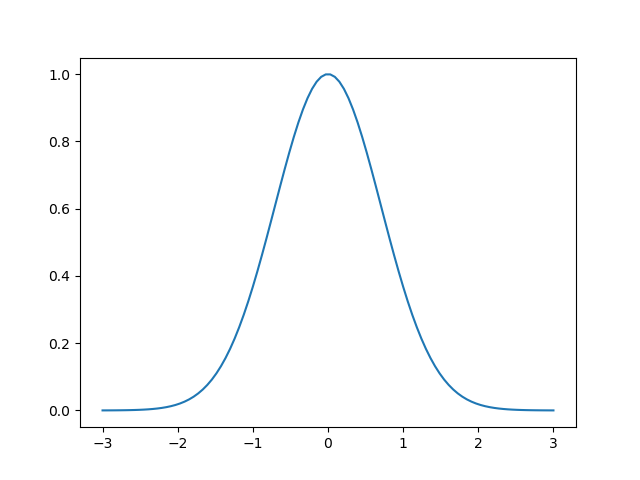
\includegraphics[scale=\myscale,scale=0.55]{figures/pythonx-gauss}
\end{center}
\end{minipage}

%--------------------------------------------------------------------
\subsection{Tracé de fonctions point par point}

Soient deux vecteurs :
\mycenterline{\ci{X = np.array([0,1,2,3,4,5])} \qquad 
\ci{Y = np.array([0,1,4,1,3,2])}}
Alors la commande \ci{plt.plot(X,Y)} affiche les points $(x,y)$ pour $x$ parcourant $X$ et $y$ parcourant $Y$ et les relie entre eux (\ci{plt} est le nom raccourci que nous avons donné au sous-module \ci{pyplot} du module \matplotlib{}). Lorsque les points sont suffisamment rapprochés cela donne l'impression d'une courbe lisse.

\index{matplotlib@\matplotlib!plot@\ci{plot()}}
\index{matplotlib@\matplotlib!scatter@\ci{scatter()}}

\begin{minipage}{0.32\textwidth}
\begin{center}
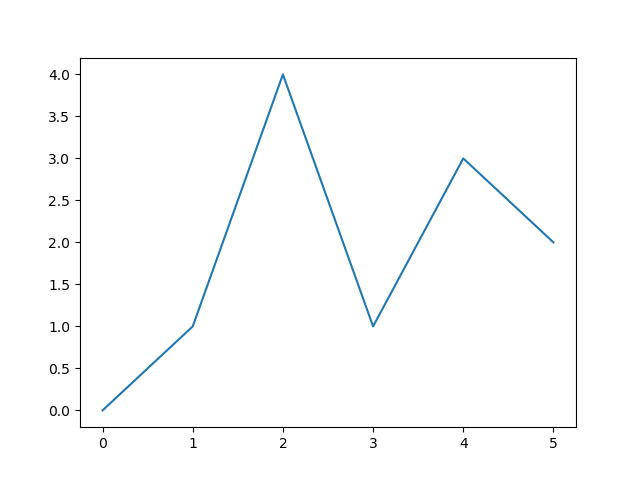
\includegraphics[scale=\myscale,scale=0.35]{figures/pythonx-plot1}
\scriptsize \ci{plt.plot(X,Y)}
\end{center}
\end{minipage}
\begin{minipage}{0.32\textwidth}
\begin{center}
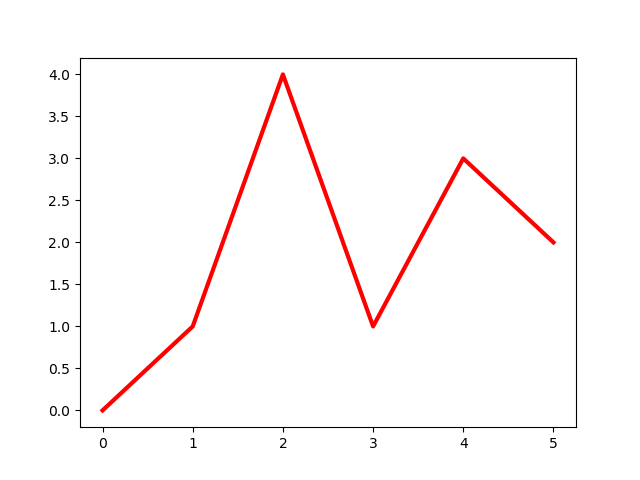
\includegraphics[scale=\myscale,scale=0.35]{figures/pythonx-plot2}
\scriptsize \ci{plt.plot(X,Y,linewidth=3,color='red')}
\end{center}
\end{minipage}
\begin{minipage}{0.32\textwidth}
\begin{center}
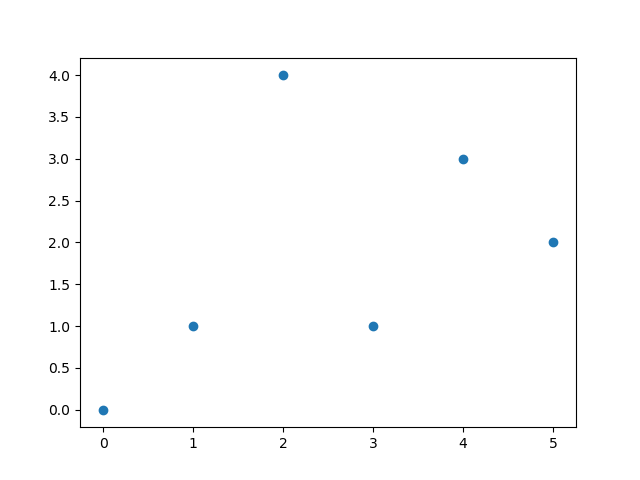
\includegraphics[scale=\myscale,scale=0.35]{figures/pythonx-plot3}
\scriptsize \ci{plt.scatter(X,Y)}
\end{center}
\end{minipage}

\bigskip

On peut bien sûr changer le style du tracé ou n'afficher que les points.


%--------------------------------------------------------------------
\subsection{Axes}

On peut exiger que le repère soit orthonormé, ajouter une grille pour plus de lisibilité.
Enfin, la commande \ci{plt.savefig()} permet de sauvegarder l'image.

\begin{minipage}{0.6\textwidth}
\begin{lstlisting}
def f(x):
	return np.exp(-x) * np.cos(2*np.pi*x)

a,b = 0,5
X = np.linspace(a,b,num=100)
Y = f(X)

plt.title('Amorti') # titre
plt.axis('equal')   # repère orthonormé
plt.grid()          # grille 
plt.xlim(a,b)       # bornes de l'axe des x
plt.plot(X,Y)
plt.savefig('amorti.png')
plt.show()
\end{lstlisting}
\end{minipage}
\begin{minipage}{0.34\textwidth}
\begin{center}
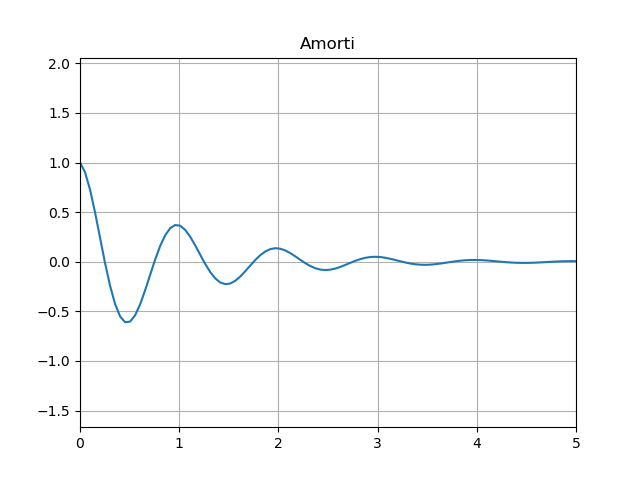
\includegraphics[scale=\myscale,scale=0.45]{figures/pythonx-amorti}
\end{center}
\end{minipage}

%--------------------------------------------------------------------
\subsection{Plusieurs tracés}

\begin{minipage}{0.4\textwidth}
On peut effectuer plusieurs tracés sur le même dessin. Ici des fonctions sigmoïdes
$$f_k(x) = \frac{1}{1+e^{-kx}}$$
avec un paramètre $k$ qui varie.
\end{minipage}
\begin{minipage}{0.59\textwidth}
\begin{center}
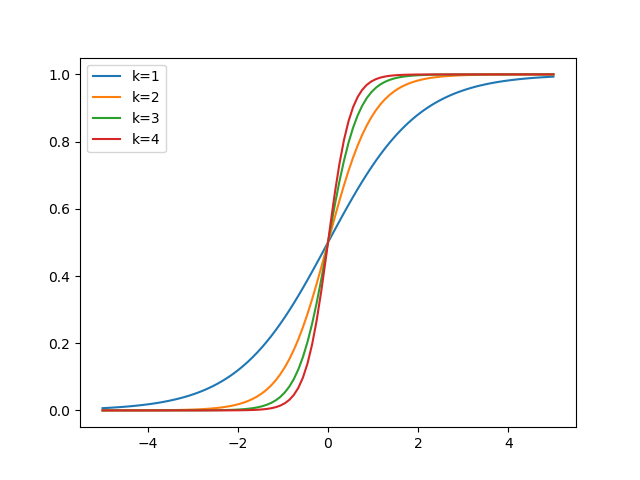
\includegraphics[scale=\myscale,scale=0.5]{figures/pythonx-sigma}
\end{center}
\end{minipage}


\begin{lstlisting}
def f(x,k):
	return 1/(1+np.exp(-k*x))

a,b = -5,5
X = np.linspace(a,b,num=100)

for k in range(1,5):
	Y = f(X,k)
	plt.plot(X,Y, label="k={}".format(k))

plt.legend()
plt.show()
\end{lstlisting}








\end{document}
